\documentclass[11pt]{article}
\usepackage[margin=0.5in]{geometry}
\usepackage{graphicx}
\usepackage{amsmath}
\usepackage{enumitem}
\usepackage{listings}

\graphicspath{{/home/konner/Documents/Stats_170/HW6/} }
\begin{document}
\centerline{\Large Stats 170 - Time Series Analysis}
\vspace{3pc}
\centerline{\Large Homework 6}
\vspace{.5pc}
\centerline{Konner Macias - 004603916}
\centerline{Dec 7th, 2018}
\vspace{1.5pc}
\section{7(b)-(e)}
\textbf{(b)} Decompose the series into the components trend, seasonal effect, and residuals, and plot the decomposed series. Produce a plot of the trend with a superimposed seasonal effect.
\\\\
\begin{center}
\textbf{Figure 1.} \\
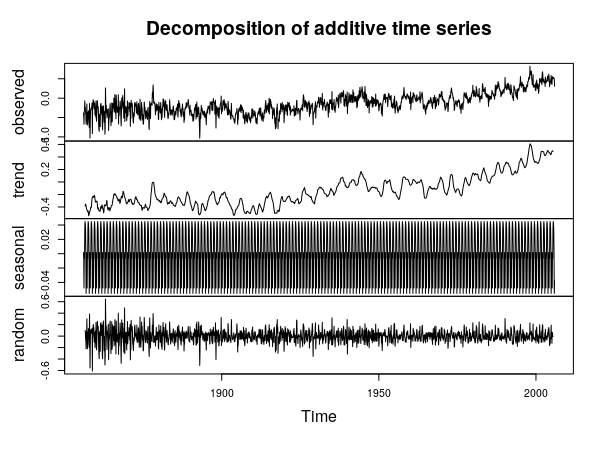
\includegraphics[scale=1]{decom} \\
\textbf{Figure 2.} \\
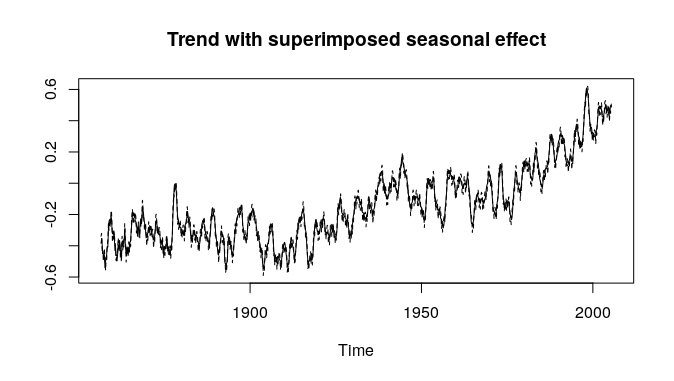
\includegraphics[scale=1]{super}
\end{center}
\textbf{(c)} Plot the correlogram of the residuals from question 7b. Comment on the plot, explaining any ‘significant’ correlations at significant lags.
\begin{center}
\textbf{Figure 3.} \\
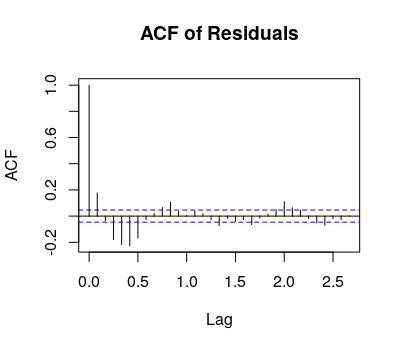
\includegraphics[scale=1]{res}
\end{center}
Figure 3 indicates that we do not have white noise residuals. There are significant correlations at lag 1, meaning that the residuals are related in some fashion to the residual one step behind it and thus is not independent. There are other correlations at lag 3,4,5, and 6 which all are negative. This is most likely due to some seasonal change within the data. Lastly, there are significant residuals at lags 9 and 10, and they are most likely positive due to a seasonal response. This sinosuidal trend continues indicating underlying seasonal effect.
\\\\
\textbf{(d)} Fit an appropriate Holt-Winters model to the monthly data. Explain why you chose that particular Holt-Winters model, and give the parameter estimates.
\\\\
I chose an additive HoltWinters model because as we noticed in Figure 1, there is an obvious trend and seasonal effect. From figure 2, we see that trend + seasonal does a fantastic job of fitting the data thus an additive model was selected. Since there is both a seasonal and trend effect, the parameters should not be zero. Here are my parameter estimates:
$$ \alpha = 0.3439351 $$
$$ \beta = 0.0004529469 $$
$$ \gamma = 0.1604094 $$
This fit has an SSE of 30.59679.
\\\\
\textbf{(e)} Using the fitted model, forecast values for the years 2005-2010. Add these forecasts to a time plot of the original series. Under what circumstances would these forecasts be valid? What comments of caution would you make to an economist or politician who wanted to use these forecasts to make statements about the potential impact of global warming on the world economy?
\begin{center}
\textbf{Figure 4.}
\\
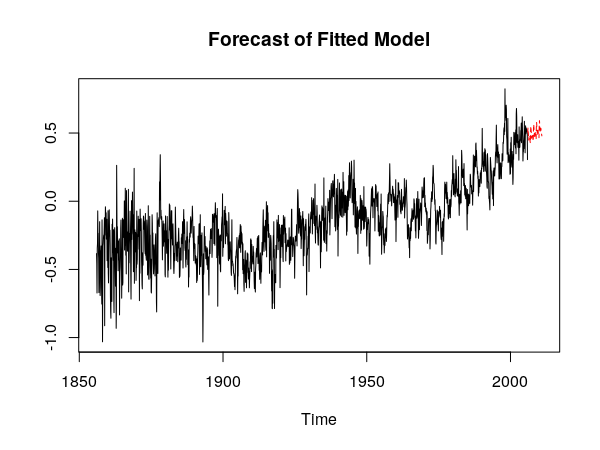
\includegraphics[scale=1]{for}
\end{center}
As long as the trend of global temperature continues without any drastic changes between 2005-2010, these forecasts are valid. A word of caution for the economist or politician would be that this model assumes a degree of statistical consistency within the data which may not hold in the real world. External factors are not taken into account, and errors could easily build and grow for forecasts over a five year period.

\section{}
Fit a state space random walk (without drift), using the code given to you in lecture for state space (also posted below).  Produce plot of the smoothing, filtering, confidence bands of the filtering. In a separate plot, plot the smoothing, the data and the forecast. Comment giving your conclusions about the fitted model for this data set. 
\begin{center}
\textbf{Figure 5.} \\
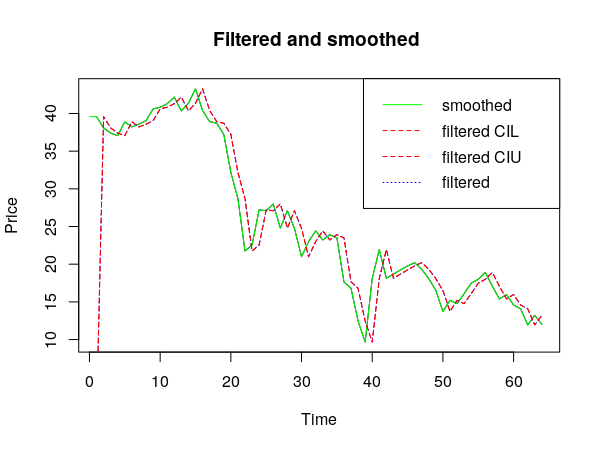
\includegraphics[scale=1]{filSmo}
\\
\textbf{Figure 6.} \\
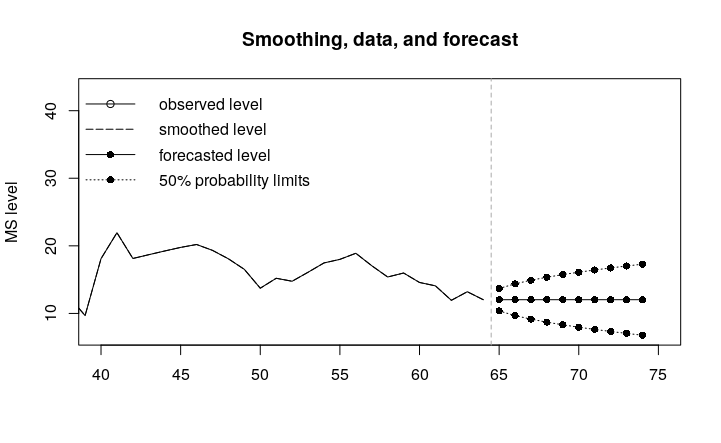
\includegraphics[scale=1]{foreSmo}
\end{center}
Looking at figure 5, the confidence bands of filtering hug the filtering value so tight that we can barely see the blue indicating a small standard error for the filtering. Looking at Figure 6, we notice that the forecasted level appears to follow the general trend for the data. We see that the probability limits get wider as time goes on. Overall, the fitted model for the data set does appear to largely capture the trend but appears to give a more smoothed estimated. This smoothed estimate makes the prediction safer by trying to generalize off of the noise of the data.
\end{document}
